%iffalse%\let\negmedspace\undefined
\let\negthickspace\undefined
\documentclass[journal,12pt,onecolumn]{IEEEtran}
\usepackage{cite}
\usepackage{amsmath,amssymb,amsfonts,amsthm}
\usepackage{algorithmic}
\usepackage{graphicx}
\usepackage{textcomp}
\usepackage{xcolor}
\usepackage{caption}
\usepackage{txfonts}
\usepackage{listings}
\usepackage{enumitem}
\usepackage{mathtools}
\usepackage{gensymb}
\usepackage{comment}
\usepackage[breaklinks=true]{hyperref}
\usepackage{tkz-euclide} 
\usepackage{listings}
\usepackage{gvv}                                        
%\def\inputGnumericTable{}                                 
\usepackage[latin1]{inputenc}   
\usepackage{xparse}
\usepackage{color}                                            
\usepackage{array}                                            
\usepackage{longtable}                                       
\usepackage{calc}                                             
\usepackage{multirow}
\usepackage{multicol}
\usepackage{hhline}                                           
\usepackage{ifthen}                                           
\usepackage{lscape}
\usepackage{tabularx}
\usepackage{array}
\usepackage{float}
\newtheorem{theorem}{Theorem}[section]
\newtheorem{problem}{Problem}
\newtheorem{proposition}{Proposition}[section]
\newtheorem{lemma}{Lemma}[section]
\newtheorem{corollary}[theorem]{Corollary}
\newtheorem{example}{Example}[section]
\newtheorem{definition}[problem]{Definition}
\newcommand{\BEQA}{\begin{eqnarray}}
\newcommand{\EEQA}{\end{eqnarray}}
\usepackage{float}
%\newcommand{\define}{\stackrel{\triangle}{=}}
\theoremstyle{remark}
\usepackage{ circuitikz }
%\newtheorem{rem}{Remark}
% Marks the beginning of the document this one
\title{ AE : AEROSPACE ENGINEERING}
\author{EE25BTECH11018-Darisy Sreetej}
\begin{document}
\maketitle

\section{GA - General Aptitude}
\textbf{Q1 - Q5 carry one mark each.}

\begin{enumerate}
   
\item The untimely loss of life is a cause of serious global concern as thousands of people get killed \dots accidents every year while many other die \dots diseases like cardio vascular disease, cancer, etc.  
\begin{enumerate}
\begin{multicols}{2}
\item in, of
\item from, of
\item during, from
\item from, from
\end{multicols}
\end{enumerate}


\item He was not only accused of theft \dots of conspiracy.  
\begin{enumerate}
\begin{multicols}{2}
\item rather
\item but also
\item but even
\item rather than
\end{multicols}
\end{enumerate}


\item Select the word that fits the analogy:  
Explicit:Implicit::Express:\dots
\begin{enumerate}
\begin{multicols}{2}
    \item Impress 
    \item Repress
    \item Compress
    \item Supress
\end{multicols}
\end{enumerate}


\item The Canadian constitution requires that equal importance be given to English and French. Last year, Air Canada lost a lawsuit, and had to pay a six-figure fine to a French-speaking couple after they filed complaints about formal in-flight announcements in English lasting 15 seconds, as opposed to informal 5 second messages in French.  
The French-speaking couple were upset at \dots
\begin{enumerate}
\item the in flight announcements being made in English
\item the English announcements being clearer than the French ones
\item the English announcements being longer than the French ones
\item equal importance being given to English and French
\end{enumerate}

\item A superadditive function $f(\cdot)$ satisfies the following property
$
    f(x_1 + x_2) \geq f(x_1) + f(x_2)
$
Which of the following functions is a superadditive function for $x > 1$?
\begin{enumerate}
\begin{multicols}{4}
    \item $e^x$
    \item $\sqrt{x}$
    \item $\dfrac{1}{x}$
    \item $e^{-x}$
    \end{multicols}
\end{enumerate}

\item The global financial crisis in 2008 is considered to be the most serious world-wide financial crisis, which started with the sub-prime lending crisis in USA in 2007. The sub-prime lending crisis led to the banking crisis in 2008 with the collapse of Lehman Brothers in 2008. The sub-prime lending refers to the provision of loans to those borrowers who may have difficulties in repaying loans, and it arises because of excess liquidity following the East Asian crisis.

Which one of the following sequences shows the correct precedence as per the given passage?
\begin{enumerate}
    \item East Asian crisis $\rightarrow$ subprime lending crisis $\rightarrow$ banking crisis $\rightarrow$ global financial crisis.
    \item Subprime lending crisis $\rightarrow$ global financial crisis $\rightarrow$ banking crisis $\rightarrow$ East Asian crisis.
    \item Banking crisis $\rightarrow$ subprime lending crisis $\rightarrow$ global financial crisis $\rightarrow$ East Asian crisis.
    \item Global financial crisis $\rightarrow$ East Asian crisis $\rightarrow$ banking crisis $\rightarrow$ subprime lending crisis.
\end{enumerate}

\item It is quarter past three in your watch. The angle between the hour hand and the minute hand is \dots.
\begin{enumerate}
\begin{multicols}{4}
    \item $0^\degree$
    \item $7.5^\degree$
    \item $15^\degree$
    \item $22.5^\degree$
    \end{multicols}
\end{enumerate}

\item A circle with centre $O$ is shown in the figure. A rectangle PQRS of maximum possible area is inscribed in the circle. If the radius of the circle is $a$, then the area of the shaded portion is \dots.

\begin{figure}[H]
    \centering
    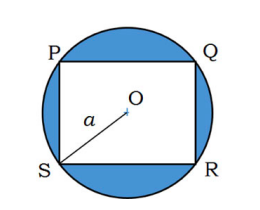
\includegraphics[width=0.5\columnwidth]{figs/Screenshot from 2025-08-17 15-20-45.png}
    \caption{Caption}
    \label{fig:placeholder}
\end{figure}

\item A circle with centre $O$ is shown in the figure. A rectangle PQRS of maximum possible area is inscribed in the circle. If the radius of the circle is $a$, then the area of the shaded portion is \dots.
\begin{enumerate}
\begin{multicols}{2}
\item $\pi a^2 - a^2$
\item $\pi a^2 - \sqrt{2} a^2$
\item $\pi a^2 - 2 a^2$
\item $\pi a^2 - 3 a^2$
\end{multicols}
\end{enumerate}

\item $a, b, c$ are real numbers. The quadratic equation $a x^2 - b x + c = 0$ has equal roots, which is $\beta$, then
\begin{enumerate}
\begin{multicols}{2}
\item $\beta = b/a$
\item $\beta^2 = ac$
\item $\beta^3 = \frac{bc}{2a^2}$
\item $b^2 \neq 4ac$
\end{multicols}
\end{enumerate}

\item The following figure shows the data of students enrolled in $5$ years (2014 to 2018) for two schools P and Q. During this period, the ratio of the average number of the students enrolled in school P to the average of the difference of the number of students enrolled in schools P and Q is \dots.
\begin{figure}[H]
    \centering
    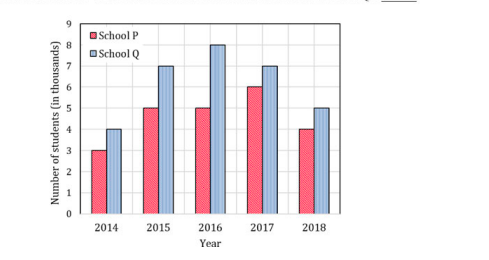
\includegraphics[width=0.5\columnwidth]{figs/Screenshot from 2025-08-17 15-29-33.png}
    \caption{Caption}
    \label{fig:placeholder}
\end{figure}
\begin{enumerate}
\begin{multicols}{4}
    \item $8 : 23$
    \item $23 : 8$
    \item $23 : 31$
    \item $31 : 23$
    \end{multicols}
\end{enumerate}
\end{enumerate}

\section{AE: Aerospace Engineering}

\textbf{Q1 - Q25 carry one mark each.}
\begin{enumerate}
   
\item For $f(x) = |x|$, with $\dfrac{df}{dx}$ denoting the derivative, the mean value theorem is not applicable because
\begin{multicols}{2}
\begin{enumerate}
    \item $f(x)$ is not continuous at $x=0$
    \item $f(x) = 0$ at $x = 0$
    \item $\dfrac{df}{dx}$ is not defined at $x = 0$
    \item $\dfrac{df}{dx} = 0$ at $x = 0$
\end{enumerate}
\end{multicols}
\hfill(GATE AE 2020)

\item For the function $f(x) = \dfrac{e^{-\lambda}}{\sigma \sqrt{2\pi}}$, where 
$\lambda = \dfrac{1}{2\sigma^2}(x-\mu)^2$, and $\sigma$ and $\mu$ are constants, the maximum occurs at
\begin{enumerate}
\begin{multicols}{2}
    \item $x = \sigma$
    \item $x = \sigma \sqrt{2\pi}$
    \item $x = 2\sigma^2$
    \item $x = \mu$
\end{multicols}
\end{enumerate}
\hfill(GATE AE 2020)


\item $y = Ae^{mx} + Be^{-mx}$, where $A$, $B$ and $m$ are constants, is a solution of
\begin{enumerate}
\begin{multicols}{2}
    \item $\dfrac{d^2 y}{dx^2} - m^2 y = 0$
    \item $A \dfrac{d^2 y}{dx^2} + m^2 y = 0$
    \item $B \dfrac{d^2 y}{dx^2} + Ay = 0$
    \item $\dfrac{d^2 y}{dx^2} + m y = m^2$
\end{multicols}
\end{enumerate}
\hfill(GATE AE 2020)

\item Which of the following statements is true about the effect of increase in temperature on dynamic viscosity of water and air, at room temperature?
\begin{enumerate}
\begin{multicols}{2}
    \item It increases for both water and air.
    \item It increases for water and decreases for air.
    \item It decreases for water and increases for air.
    \item It decreases for both water and air.
\end{multicols}
\end{enumerate}
\hfill(GATE AE 2020)

\item Given access to the complete geometry, surface pressure and shear stress distribution over a body placed in a uniform flow, one can estimate
\begin{enumerate}
    \item the moment coefficient, and the force on the body.
    \item the force coefficient, and the force on the body.
    \item the moment coefficient, and the moment on the body.
    \item the force and the moment on the body.
\end{enumerate}
\hfill(GATE AE 2020)

\item A pair of infinitely long, counter-rotating line vortices of the same circulation strength $\Gamma$ are situated a distance $h$ apart in a fluid, as shown in the figure. The vortices will
\begin{figure}[H]
    \centering
    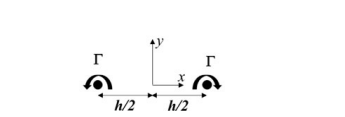
\includegraphics[width=0.5\columnwidth]{figs/Screenshot from 2025-08-17 15-53-02.png}
    \caption{Caption}
    \label{fig:placeholder}
\end{figure}
\begin{enumerate}
    \item rotate counter-clockwise about the midpoint with the tangential velocity at the line vortex equal to $\dfrac{\Gamma}{2 \pi h}$
    \item rotate counter-clockwise about the midpoint with the tangential velocity at the line vortex equal to $\dfrac{\Gamma}{4 \pi h}$
    \item translate along $+y$ direction with velocity at the line vortex equal to $\dfrac{\Gamma}{2 \pi h}$
    \item translate along $+y$ direction with velocity at the line vortex equal to $\dfrac{\Gamma}{4 \pi h}$
\end{enumerate}
\hfill(GATE AE 2020)

\item The streamlines of a steady two dimensional flow through a channel of height $0.2$ m are plotted in the figure, where $\Psi$ is the stream function in m$^2$/s. The volumetric flow rate per unit depth is \dots.
\begin{figure}[H]
    \centering
    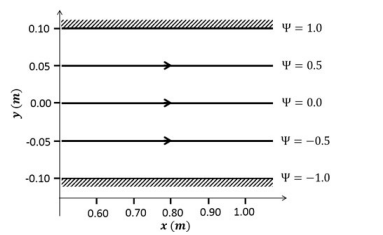
\includegraphics[width=0.5\columnwidth]{figs/Screenshot from 2025-08-17 15-59-39.png}
    \caption{Caption}
    \label{fig:placeholder}
\end{figure}
The volumetric flow rate per unit depth is \dots.
    \begin{enumerate}
    \begin{multicols}{4}
        \item $1.0$ m$^2$/s
        \item $2.0$ m$^2$/s
        \item $0.5$ m$^2$/s
        \item $0.1$ m$^2$/s
        \end{multicols}
    \end{enumerate}
    \hfill(GATE AE 2020)

\item Which of the following options can result in an increase in the Mach number of a supersonic flow in a duct?
    \begin{enumerate}
        \item Increasing the length of the duct
        \item Adding heat to the flow
        \item Removing heat from the flow
        \item Inserting a convergent-divergent section with the same cross-sectional area at its inlet and exit planes
    \end{enumerate}
    \hfill(GATE AE 2020)

\item Which one of the following conditions needs to be satisfied for
    $
        \phi = Ax^4 + By^4 + Cx y^3
    $
    to be considered as an Airy's stress function?
    \begin{enumerate}
    \begin{multicols}{2}
        \item $A - B = 0$
        \item $A + B = 0$
        \item $A - C = 0$
        \item $A + C = 0$
          \end{multicols}
    \end{enumerate}
    \hfill(GATE AE 2020)

\item Consider the plane strain field given by $\varepsilon_{xx} = Ay^2 + x$, $\varepsilon_{yy} = Ax^2 + y$, $\gamma_{xy} = B x y + y$. The relation between $A$ and $B$ needed for this strain field to satisfy the compatibility condition is
    \begin{enumerate}
    \begin{multicols}{4}
        \item $B = A$
        \item $B = 2A$
        \item $B = 3A$
        \item $B = 4A$
         \end{multicols}
    \end{enumerate}
    \hfill(GATE AE 2020)

\item For hyperbolic trajectory of a satellite of mass $m$ having velocity $V$ at a distance $r$ from the center of earth ($G$: gravitational constant, $M$: mass of earth), which one of the following relations is true?
    \begin{enumerate}
    \begin{multicols}{2}    
        \item $\dfrac{1}{2} mV^2 < \dfrac{GMm}{r}$
        \item $\dfrac{1}{2} mV^2 < \dfrac{GMm}{r}$
        \item $\dfrac{1}{2} mV^2 = \dfrac{GMm}{r}$
        \item $\dfrac{1}{2} mV^2 > \dfrac{GMm}{r}$
        \end{multicols}
    \end{enumerate}
    \hfill(GATE AE 2020)

\item For conventional airplanes, which one of the following is true regarding roll control derivative $\left( C_{l_{\delta_r}} = \frac{\partial C_l}{\partial \delta_r} \right)$ and yaw control derivative $\left( C_{n_{\delta_r}} = \frac{\partial C_n}{\partial \delta_r} \right)$, where $\delta_r$ is rudder deflection?
\begin{enumerate}
    \begin{multicols}{2}
        \item $C_{l_{\delta_r}} > 0 $ and $C_{n_{\delta_r}} < 0$
        \item $C_{l_{\delta_r}} < 0 $ and $C_{n_{\delta_r}} > 0$
        \item $C_{l_{\delta_r}} < 0 $ and $C_{n_{\delta_r}} < 0$
        \item $C_{l_{\delta_r}} > 0 $ and $C_{n_{\delta_r}} > 0$
    \end{multicols}
\end{enumerate}
\hfill(GATE AE 2020)

\item The ratio of exit stagnation pressure to inlet stagnation pressure across the rotating impeller of a centrifugal compressor, operating with a closed exit, is
\begin{enumerate}
    \begin{multicols}{4}
        \item 0
        \item 1
        \item $>$ 1
        \item 0.5
    \end{multicols}
\end{enumerate}
\hfill(GATE AE 2020)

\item Which one of the following is a hypergolic propellant combination used in rocket engines?
\begin{enumerate}
        \item Liquid hydrogen -- liquid oxygen
        \item Unsymmetrical dimethyl hydrazine -- nitrogen tetroxide
        \item Rocket fuel RP-1 -- liquid oxygen
        \item Liquid hydrogen -- liquid fluorine
\end{enumerate}
\hfill(GATE AE 2020)

\item In aircraft engine thermodynamic cycle analysis, \textit{perfectly expanded flow} in the nozzle means that the static pressure in the flow at the nozzle exit is equal to
\begin{enumerate}
    \begin{multicols}{2}
        \item the stagnation pressure at the engine inlet.
        \item the stagnation pressure at the nozzle exit.
        \item the ambient pressure at the nozzle exit.
        \item the static pressure at the nozzle inlet.
    \end{multicols}
\end{enumerate}
\hfill(GATE AE 2020)

\item Three long and slender aluminum bars of identical length are subjected to an axial tensile force. These bars have circular, triangular and rectangular cross sections, with same cross sectional area. If they yield at $F_{circle}$, $F_{triangle}$ and $F_{rectangle}$, respectively, which one of the following is true?
\begin{enumerate}
    \begin{multicols}{2}
        \item $F_{circle} > F_{triangle} > F_{rectangle}$
        \item $F_{circle} < F_{triangle} < F_{rectangle}$
        \item $ F_{triangle} >F_{circle} > F_{rectangle}$
        \item $F_{circle} = F_{triangle} = F_{rectangle}$
    \end{multicols}
\end{enumerate}
\hfill(GATE AE 2020)

\item The positive high angle-of-attack condition is obtained in a steady pull-out maneuver at the largest permissible angle-of-attack of the wing. Under this condition, at which of the following regions of the wing does the maximum tension occur?
   \begin{figure}[H]
       \centering
       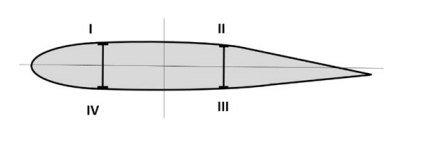
\includegraphics[width=0.5\columnwidth]{figs/Screenshot from 2025-08-18 15-24-29.png}
       \caption{Caption}
       \label{fig:placeholder}
   \end{figure}
\begin{enumerate}
    \begin{multicols}{4}
        \item I
        \item II
        \item III
        \item IV
    \end{multicols}
\end{enumerate}
\hfill(GATE AE 2020)

\item The natural frequency of the first mode of a rectangular cross section cantilever aluminum beam is $\omega$ rad/s. If the material and cross-section remain the same, but the length of the beam is doubled, the first mode frequency will become
\begin{enumerate}
    \begin{multicols}{4}
        \item $\frac{\omega}{4} \text{ rad/s}$
        \item $4\omega \text{ rad/s}$
        \item $\frac{\omega}{16} \text{ rad/s}$
        \item $16\omega \text{ rad/s}$
    \end{multicols}
\end{enumerate}
\hfill(GATE AE 2020)

\item Given $A = \myvec{ \sin\theta & \tan\theta \\ 0 & \cos\theta }$, the sum of squares of eigenvalues of $A$ is
\begin{enumerate}
    \begin{multicols}{4}
        \item $\tan^2 \theta$
        \item $1$
        \item $\sin^2 \theta$
        \item $\cos^2 \theta$
    \end{multicols}
\end{enumerate}
\hfill(GATE AE 2020)

\item Burnout velocity of a space vehicle in a circular orbit at an angle $5^\degree$ above the local horizon around earth is $13.5$ km/s. Tangential velocity of the space vehicle in the orbit is \dots km/s \textit{(round off to two decimal places)}.
\hfill(GATE AE 2020)

\item Velocity of an airplane in the body fixed axes is given as $[100 \quad -10 \quad 20]$ m/s. The sideslip angle is \dots degrees \textit{(round off to two decimal places)}.
\hfill(GATE AE 2020)

\item The similarity solution for the diffusion equation, 
$
\frac{\partial u}{\partial t} = a \frac{\partial^2 u}{\partial x^2}
$
is $u(x, \eta) = u(\eta)$, where similarity variable, $\eta = \frac{x}{\sqrt{a t}}$. If $u(x, 0) = e^{-x^2}$, the ratio $\frac{u(0, 1)}{u(0, 4)} =$ \dots \textit{(round off to one decimal place).}
\hfill(GATE AE 2020)

\item Air enters the rotor of an axial compressor stage with no pre-whirl ($C_{\theta} = 0$) and exits the rotor with whirl velocity, $C_{\theta} = 150$ m/s. The velocity of rotor vanes, $U$ is 200 m/s. Assuming $C_p = 1005$ J/(kg·K), the stagnation temperature rise across the rotor is \dots K \textit{(round off to one decimal place).}
\hfill(GATE AE 2020)

\item A thin walled beam of constant thickness shown in the figure is subjected to a torque of $3.2$ kNm. If the shear modulus is $25$ GPa, the angle of twist per unit length is \dots rad/m \textit{(round off to three decimal places).}
\hfill(GATE AE 2020)

\begin{figure}[H]
    \centering
    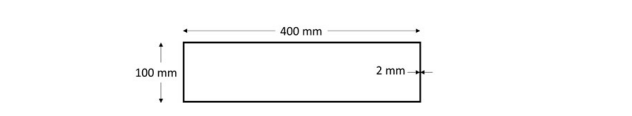
\includegraphics[width=0.5\columnwidth]{figs/Screenshot from 2025-08-18 15-35-45.png}
    \caption{Caption}
    \label{fig:placeholder}
\end{figure}

\item An airplane of mass 5000 kg is flying at a constant speed of 360 km/h at the bottom of a vertical circle with a radius of 400 m, as shown in the figure. Assuming that the acceleration due to gravity is $9.8$ m/s$^2$, the load factor experienced at the center of gravity of the airplane is \dots. \textit{(round off to two decimal places).}

\begin{figure}[H]
    \centering
    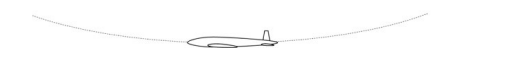
\includegraphics[width=0.5\columnwidth]{figs/Screenshot from 2025-08-18 15-37-45.png}
    \caption{Caption}
    \label{fig:placeholder}
\end{figure}
 \hfill(GATE AE 2020)

\textbf{Q26 - Q55 carry two marks each.}
\item The equation $x \frac{dx}{dy} + y = c$, where $c$ is a constant, represents a family of
\begin{enumerate}
    \begin{multicols}{2}
        \item exponential curves
        \item parabolas
        \item circles
        \item hyperbolas
    \end{multicols}
\end{enumerate}
\hfill(GATE AE 2020)

\item A wedge shaped airfoil is placed in a supersonic flow as shown in the figure (not to scale). The corners of the wedge are at $x = x_A$, $x = x_B$, $x = x_C$, respectively.

\begin{figure}[H]
    \centering
    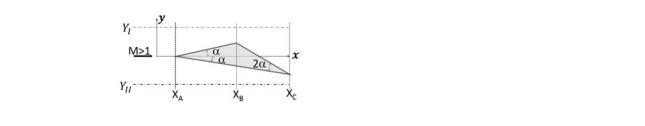
\includegraphics[width=0.5\columnwidth]{figs/Screenshot from 2025-08-18 15-46-10.png}
    \caption{Caption}
    \label{fig:placeholder}
\end{figure}
 
Which one of the following represents the correct static pressure profiles along $y = y_I$ and $y = y_{II}$?
\begin{enumerate}
  
        \item 
        \begin{figure}[H]
            \centering
            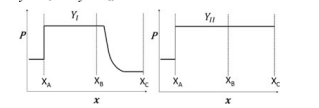
\includegraphics[width=0.5\columnwidth]{figs/Screenshot from 2025-08-18 16-01-49.png}
            \caption{Caption}
            \label{fig:placeholder}
        \end{figure}
        
        \item 
        \begin{figure}[H]
            \centering
            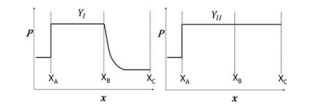
\includegraphics[width=0.5\columnwidth]{figs/Screenshot from 2025-08-18 16-03-56.png}
            \caption{Caption}
            \label{fig:placeholder}
        \end{figure}
        
        \item 
        \begin{figure}[H]
            \centering
            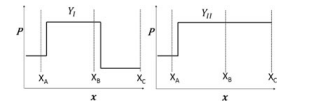
\includegraphics[width=0.5\columnwidth]{figs/Screenshot from 2025-08-18 16-07-16.png}
            \caption{Caption}
            \label{fig:placeholder}
        \end{figure}
        \item 
        \begin{figure}[H]
            \centering
            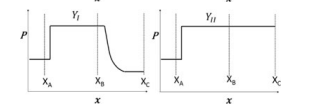
\includegraphics[width=0.5\columnwidth]{figs/Screenshot from 2025-08-18 16-11-15.png}
            \caption{Caption}
            \label{fig:placeholder}
        \end{figure}
\end{enumerate}
\hfill(GATE AE 2020)

\item The value of Poisson's ratio at which the shear modulus of an isotropic material is equal to the bulk modulus is
\begin{enumerate}
    \begin{multicols}{4}
        \item $\dfrac{1}{2}$
        \item $\dfrac{1}{4}$
        \item $\dfrac{1}{6}$
        \item $\dfrac{1}{8}$
    \end{multicols}
\end{enumerate}
\hfill(GATE AE 2020)

\item A load $P$ is applied to the free end of a stepped cantilever beam as shown in the figure. The Young's modulus of the material is $E$, and the moments of inertia of the two sections of length $2\,\text{m}$ and $1\,\text{m}$ are $I$ and $3I$, respectively. Ignoring transverse shear and stress concentration effects, the deflection at the point where the load is applied at the free end of the cantilever is

\begin{figure}[H]
    \centering
    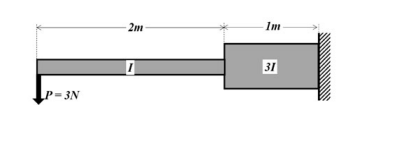
\includegraphics[width=0.5\columnwidth]{figs/Screenshot from 2025-08-19 15-28-06.png}
    \caption{Caption}
    \label{fig:placeholder}
\end{figure}


\begin{enumerate}
\begin{multicols}{4}
  \item $\dfrac{23}{243EI}$
  \item $\dfrac{1}{3EI}$
  \item $\dfrac{43}{3EI}$
  \item $\dfrac{23}{3EI}$
\end{multicols}
\end{enumerate}
\hfill(GATE AE 2020)

\ The three dimensional strain-stress relation for an isotropic material, written in a general matrix form, is

$
\myvec{
\epsilon_{xx} \\
\epsilon_{yy} \\
\epsilon_{zz} \\
\gamma_{xy} \\
\gamma_{xz} \\
\gamma_{yz}
}
=
\myvec{
A & C & C & 0 & 0 & 0 \\
C & A & C & 0 & 0 & 0 \\
C & C & A & 0 & 0 & 0 \\
0 & 0 & 0 & B & 0 & 0 \\
0 & 0 & 0 & 0 & B & 0 \\
0 & 0 & 0 & 0 & 0 & B
}
\myvec{
\sigma_{xx} \\
\sigma_{yy} \\
\sigma_{zz} \\
\tau_{xy} \\
\tau_{xz} \\
\tau_{yz}
}
$

$A$, $B$ and $C$ are compliances which depend on the elastic properties of the material.

Which one of the following is correct?

\begin{enumerate}
\begin{multicols}{2}
  \item $C = \dfrac{A}{2} - B$
  \item $C = \dfrac{A}{2} + B$
  \item $C = A + \dfrac{B}{2}$
  \item $C = A - \dfrac{B}{2}$
\end{multicols}
\end{enumerate}
\hfill(GATE AE 2020)

\item For three different airplanes A, B and C, the yawing moment coefficient ($C_n$) was measured in a wind-tunnel for three settings of sideslip angle $\beta$ and tabulated as

\begin{tabular}[12pt]{ |c| c| c| c| }
\hline
$\beta$ & Airplane A & Airplane B & Airplane C \\
\hline
$\beta = -5\,\mathrm{deg}$ & $-0.030$ & $-0.025$ & $0.040$\\
\hline
$\beta = 0\,\mathrm{deg}$ & $0$ & $0$ & $0$ \\
\hline
$\beta = 5\,\mathrm{deg}$ & $0.030$ & $0.025$ & $-0.040$\\
\hline
\end{tabular}


Which one of the following statements is true regarding directional static stability of the airplanes A, B and C?
\begin{enumerate}
    \item All three airplanes A, B, and C are stable.
    \item Only airplane C is stable, while both A and B are unstable.
    \item Airplane C is unstable, A and B are stable with A being more stable than B.
    \item Airplane C is unstable, A and B are both stable with A less stable than B.
\end{enumerate}
\hfill(GATE AE 2020)

\item A closed curve is expressed in parametric form as $x = a \cos \theta$ and $y = b \sin \theta$, where $a = 7$\,m and $b = 5$\,m. Approximating $\pi = \frac{22}{7}$, which of the following is the area enclosed by the curve?
\begin{enumerate}
\begin{multicols}{2}
    \item 110\,m$^2$
    \item 74\,m$^2$
    \item 35\,m$^2$
    \item 144\,m$^2$
    \end{multicols}
\end{enumerate}
\hfill(GATE AE 2020)

\item An axial compressor is designed to operate at a rotor speed of 15000\,rpm and an inlet stagnation temperature of 300\,K. During compressor testing, the inlet stagnation temperature of the compressor measured was 280\,K. What should be the rotor speed for the compressor to develop the same performance characteristics during this test as in the design condition?
\begin{enumerate}
\begin{multicols}{2}
    \item 14000\,rpm
    \item 14491\,rpm
    \item 15526\,rpm
    \item 16071\,rpm
    \end{multicols}
\end{enumerate}
\hfill(GATE AE 2020)

\item For the state of stress shown in the figure, which one of the following represents the correct free body diagram showing the maximum shear stress and the associated normal stresses?

\begin{figure}[H]
    \centering
    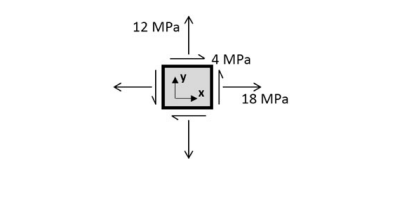
\includegraphics[width=0.5\columnwidth]{figs/Screenshot from 2025-08-19 15-40-59.png}
    \caption{Caption}
    \label{fig:placeholder}
\end{figure}

\begin{enumerate}
  

\item 
\begin{figure}[H]
    \centering
    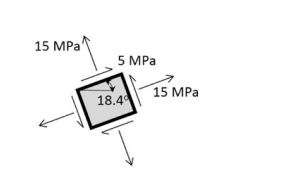
\includegraphics[width=0.5\columnwidth]{figs/Screenshot from 2025-08-19 15-42-35.png}
    \caption{Caption}
    \label{fig:placeholder}
\end{figure}
\item 
\begin{figure}[H]
    \centering
    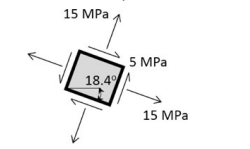
\includegraphics[width=0.5\columnwidth]{figs/Screenshot from 2025-08-19 15-44-14.png}
    \caption{Caption}
    \label{fig:placeholder}
\end{figure}
 \item 
 \begin{figure}[H]
     \centering
     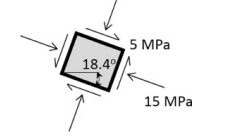
\includegraphics[width=0.5\columnwidth]{figs/Screenshot from 2025-08-19 15-45-13.png}
     \caption{Caption}
     \label{fig:placeholder}
 \end{figure}
 \item 
 \begin{figure}[H]
     \centering
     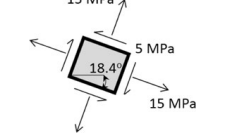
\includegraphics[width=0.5\columnwidth]{figs/Screenshot from 2025-08-19 15-46-00.png}
     \caption{Caption}
     \label{fig:placeholder}
 \end{figure}
\end{enumerate}
\hfill(GATE AE 2020)


\item In the equation $AX = B$, 
$
A = \myvec{
\dfrac{1}{\sqrt{2}} & 0 & \dfrac{1}{\sqrt{2}} \\
0 & 1 & 0 \\
\dfrac{1}{\sqrt{2}} & 0 & -\dfrac{1}{\sqrt{2}}
},
\quad
X = \myvec{
x \\
y \\
z
},
\quad
B = \myvec{
0 \\
1 \\
-\sqrt{2}
}
$
where $A$ is an orthogonal matrix, the sum of the unknowns, $x + y + z =$ \dots. \textit{(round off to one decimal place).}
\hfill(GATE AE 2020)

\item If $\int_{0}^{1} (x^2 - 2x + 1)\, dx$ is evaluated numerically using trapezoidal rule with four intervals, the difference between the numerically evaluated value and the analytical value of the integral is equal to \dots. \textit{ (round off to three decimal places).}
\hfill(GATE AE 2020)

\item The table shows the lift characteristics of an airfoil at low speeds. The maximum lift coefficient occurs at 16 degrees.

\begin{center}
\begin{tabular}{|p{1cm}|p{3cm}|p{1cm}|p{7cm}|}
\hline

\multicolumn{2}{|c|}{Process} & \multicolumn{2}{c|}{Application} \\
\hline
P & Extrusion & 1 & Producing complex parts with close tolerance \\
\hline
Q & Injection molding & 2 & Producing thermosetting plastic components \\
\hline
R & Blow molding & 3 & Producing long uniform sections \\
\hline
S & Compression molding & 4 & Producing hollow shapes \\
\hline
\end{tabular}
\end{center}
\hfill(GATE AE 2020)

Using Prandtl-Glauret rule, the lift coefficient for the airfoil at the angle of attack of 6 degrees and free stream Mach number of 0.6 is \dots \textit{(round off to two decimal places).}
\hfill(GATE AE 2020)

\item A low speed uniform flow $U_0$ is incident on an airfoil of chord $c$. In the figure, the velocity profile some distance downstream of the airfoil is idealized as shown for section B. The static pressure at sections A and B is the same. The drag coefficient of the airfoil is \dots \textit{(round off to three decimal places).}
\hfill(GATE AE 2020)

\item A low speed uniform flow $U_0$ is incident on an airfoil of chord $c$. In the figure, the velocity profile some distance downstream of the airfoil is idealized as shown for section B. The static pressure at sections A and B is the same. The drag coefficient of the airfoil is \dots \textit{(round off to three decimal places).}

\begin{figure}[H]
    \centering
    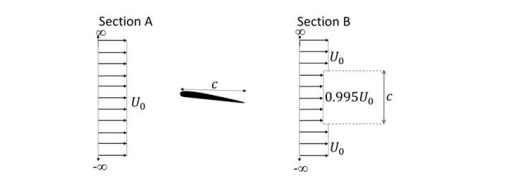
\includegraphics[width=0.5\columnwidth]{figs/Screenshot from 2025-08-19 15-56-20.png}
    \caption{Caption}
    \label{fig:placeholder}
\end{figure}
\hfill(GATE AE 2020)

\item An oblique shock is inclined at an angle of 35 degrees to the upstream flow of velocity 517.56\,m/s. The deflection of the flow due to this shock is 5.75 degrees and the temperature downstream is 182.46\,K. Assume the gas constant $R = 287\,\text{J/(kg\,K)}$, specific heat ratio $\gamma = 1.4$, and specific heat at constant pressure $C_p = 1005\,\text{J/(kg\,K)}$. Using conservation relations, the Mach number of the upstream flow can be obtained as \dots.  \textit{(round off to one decimal place).}
\hfill(GATE AE 2020)

\item The thickness of a laminar boundary layer ($\delta$) over a flat plate is,
$
\frac{\delta}{x} = \frac{5.2}{\sqrt{Re_x}},
$
where $x$ is measured from the leading edge along the length of the plate. The velocity profile within the boundary layer is idealized as varying linearly with $y$. For freestream velocity of 3\,m/s and kinematic viscosity of $1.5 \times 10^{-5}\,\text{m}^2/\text{s}$, the displacement thickness at 0.5\,m from the leading edge is \dots mm. \textit{(round off to two decimal places).}
\hfill(GATE AE 2020)

\item A wing of 15\,m span with elliptic lift distribution is generating a lift of 80\,kN at a speed of 90\,m/s. The density of surrounding air is 1.2\,kg/m$^3$. The induced angle of attack at this condition is \dots degrees. \textit{(round off to two decimal places).}
\hfill(GATE AE 2020)

\item A solid circular shaft, made of ductile material with yield stress $\sigma_Y = 280\,\text{MPa}$, is subjected to a torque of 10\,kNm. Using the Tresca failure theory, the smallest radius of the shaft to avoid failure is \dots cm. \textit{(round off to two decimal places).}
\hfill(GATE AE 2020)

\item The ratio of tangential velocities of a planet at the perihelion and the aphelion from the sun is $1.0339$. Assuming that the planet's orbit around the sun is planar and elliptic, the value of eccentricity of the orbit is \dots. \textit{(round off to three decimal places).}
\hfill(GATE AE 2020)

\item The eigenvalues for phugoid mode of a general aviation airplane at a stable cruise flight condition at low angle of attack are $\lambda_{1,2} = -0.02 \pm i\,0.25$. If the acceleration due to gravity is $9.8\,\text{m/s}^2$, the equilibrium speed of the airplane is \dots \text{m/s}. \textit{(round off to two decimal places).}
\hfill(GATE AE 2020)

\item For a general aviation airplane with tail efficiency $\eta = 0.95$, horizontal tail volume ratio $V_{H} = 0.453$, downwash angle slope $\dfrac{d\epsilon}{d\alpha} = 0.35$, wing lift curve slope $C'_{L\alpha^w} = 4.8\,\text{rad}^{-1}$, horizontal tail lift curve slope $C'_{L\alpha^t} = 4.4\,\text{rad}^{-1}$, shift in neutral point location as a percentage of mean aerodynamic chord is \dots. \text{(round off to two decimal places).}
\hfill(GATE AE 2020)

\item A single engine, propeller driven, general aviation airplane is flying in cruise at sea-level condition (density of air at sea-level is $1.225\,\text{kg/m}^3$) with speed to cover maximum range. For drag coefficient $C_D = 0.025 + 0.049\,C_L^2$ and wing loading $W/S = 9844\,\text{N/m}^2$, the speed of the airplane is \dots \text{m/s}. \textit{(round off to one decimal place).}
\hfill(GATE AE 2020)

\item The design flight Mach number of an ideal ramjet engine is $2.8$. The stagnation temperature of air at the exit of the combustor is $2400\,\text{K}$. Assuming the specific heat ratio of $1.4$ and gas constant of $287\,\text{J/(kg\,K)}$, the velocity of air at the exit of the engine is \dots \text{m/s}. \textit{(round off to one decimal place).}
\hfill(GATE AE 2020)

\item The operating conditions of an aircraft engine combustor are as follows. The rate of total enthalpy of air entering the combustor $= 28.94\,\text{MJ/s}$. The rate of total enthalpy of air leaving the combustor $= 115.42\,\text{MJ/s}$. Mass flow rate of air $= 32\,\text{kg/s}$. Air to fuel mass ratio $= 15.6$. Lower heating value of the fuel $= 46\,\text{MJ/kg}$. 
The efficiency of the combustor is \dots. \textit{(round off to two decimal places).}
\hfill(GATE AE 2020)

\item The figure shows the T-S diagram for an axial turbine stage.

\begin{figure}[H]
    \centering
    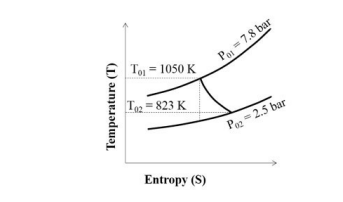
\includegraphics[width=0.5\columnwidth]{figs/Screenshot from 2025-08-19 16-14-00.png}
    \caption{Caption}
    \label{fig:placeholder}
\end{figure}

Assuming specific heat ratio of 1.33 for the hot gas, the isentropic efficiency of the turbine stage is \dots. \textit{(round off to two decimal places).}
\hfill(GATE AE 2020)

\item A rocket engine has a sea level specific impulse of 210\,s and a nozzle throat area of 0.005\,m$^2$. While testing at sea level conditions, the characteristic velocity and pressure for the thrust chamber are 1900\,m/s and 50\,bar, respectively. Assume the acceleration due to gravity to be 9.8\,m/s$^2$. The thrust produced by the rocket engine is \dots kN. \textit{(round off to one decimal place).}
\hfill(GATE AE 2020)

\item A critically damped single degree of freedom spring-mass-damper system used in a door closing mechanism becomes overdamped due to softening of the spring with extended use. If the new damping ratio ($\xi_\text{new}$) for overdamped condition is 1.2, the ratio of the original spring stiffness to the new spring stiffness ($k_\text{org} / k_\text{new}$), assuming that the other parameters remain unchanged, is \dots \textit{(round off to two decimal places).}
\hfill(GATE AE 2020)

\item The two masses of the two degree of freedom system shown in the figure are given initial displacements of 2\,cm ($x_1$) and 1.24\,cm ($x_2$). The system starts to vibrate in the first mode. The first mode shape of this system is $\phi = [1~a]^T$, where $a =$ \dots \textit{(round off to two decimal places).}

\begin{figure}[H]
    \centering
    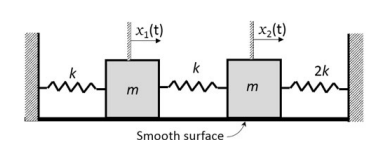
\includegraphics[width=0.5\columnwidth]{figs/Screenshot from 2025-08-19 16-16-27.png}
    \caption{Caption}
    \label{fig:placeholder}
\end{figure}
\hfill(GATE AE 2020)

\item As shown in the figure, a beam of length $1\,\mathrm{m}$ is rigidly supported at one end and simply supported at the other. Under the action of a uniformly distributed load of $10\,\mathrm{N/m}$, the magnitude of the normal reaction force at the simply supported end is \dots $\mathrm{N}$ \textit{(round off to two decimal places).}

\begin{figure}[H]
    \centering
    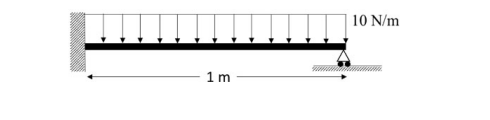
\includegraphics[width=0.5\columnwidth]{figs/Screenshot from 2025-08-19 16-20-40.png}
    \caption{Caption}
    \label{fig:placeholder}
\end{figure}
\hfill(GATE AE 2020)

\item An airplane of mass $4000\,\mathrm{kg}$ and wing reference area $25\,\mathrm{m^2}$ flying at sea level has a maximum lift coefficient of $1.65$. Assume density of air as $1.225\,\mathrm{kg/m^3}$ and acceleration due to gravity as $9.8\,\mathrm{m/s^2}$. Using a factor of safety of $1.25$ to account for additional unsteady lift during a sudden pull-up, the speed at which the airplane reaches a load factor of $3.2$ is \dots $\mathrm{m/s}$ \textit{(round off to two decimal places).}
\hfill(GATE AE 2020)

\item A Pitot tube mounted on the wing tip of an airplane flying at an altitude of $3\,\mathrm{km}$ measures a pressure of $0.72\,\mathrm{bar}$, and the outside air temperature is $268.66\,\mathrm{K}$. Take the sea level conditions as: pressure $= 1.01\,\mathrm{bar}$, temperature $= 288.16\,\mathrm{K}$, and density $= 1.225\,\mathrm{kg/m^3}$. The acceleration due to gravity is $9.8\,\mathrm{m/s^2}$ and the gas constant is $287\,\mathrm{J/(kg\,K)}$. Assuming standard atmosphere, the equivalent airspeed for this airplane is \dots $\mathrm{m/s}$ \textit{(round off to two decimal place).}
\hfill(GATE AE 2020)

\newpage

\begin{table}[h!]
\small
\setlength{\tabcolsep}{4pt}
\renewcommand{\arraystretch}{0.9}
\centering
\begin{tabular}{|c|c|c|p{1.8cm}|p{2.5cm}|c|}
\hline
Q. No & Type & Section & Key & Marks \\
\hline
1  & MCQ & GA & C         & 1 \\
\hline
2  & MCQ & GA & A         & 1 \\
\hline
3  & MCQ & GA & A         & 1 \\
\hline
4  & MCQ & GA & A         & 1 \\
\hline
5  & MCQ & GA & D         & 1 \\
\hline
6  & MCQ & GA & D         & \textbf{2} \\
\hline
7  & MCQ & GA & B         & 2 \\
\hline
8  & MCQ & GA & C         & 2 \\
\hline
9  & MCQ & GA & B         & 2 \\
\hline
10 & MCQ & GA & C         & 2 \\
\hline
11 & MCQ & EY & D         & 1 \\
\hline
12 & MCQ & EY & D         & 1 \\
\hline
13 & MCQ & EY & A; D      & 1 \\
\hline
14 & MCQ & EY & B         & 1 \\
\hline
15 & NAT & EY & 7.99 : 8.10 & 1 \\
\hline
16 & MCQ & EY & B         & 1 \\
\hline
17 & MCQ & EY & C         & 1 \\
\hline
18 & MCQ & EY & D         & 1 \\
\hline
19 & NAT & EY & 9.9 : 10.1  & 1 \\
\hline
20 & MCQ & EY & C         & 1 \\
\hline
21 & MCQ & EY & B         & 1 \\
\hline
22 & MCQ & EY & A         & 1 \\
\hline
23 & MCQ & EY & D         & 1 \\
\hline
24 & MCQ & EY & B         & 1 \\
\hline
25 & MCQ & EY & A         & 1 \\
\hline
26 & MCQ & EY & C         & 2 \\
\hline
27 & MCQ & EY & D         & 2 \\
\hline
28 & MCQ & EY & C         & 2 \\
\hline
29 & MCQ & EY & D         & 2 \\
\hline
30 & MCQ & EY & B         & 2 \\
\hline
31 & MCQ & EY & A         & 2 \\
\hline
32 & MCQ & EY & C         & 2 \\
\hline
33 & MCQ & EY & A         & 2 \\
\hline
34 & MCQ & EY & B         & 2 \\
\hline
35 & MCQ & EY & A         & 2 \\
\hline
36 & MCQ & EY & A         & 2 \\
\hline
37 & MCQ & EY & C         & 2 \\
\hline
38 & MCQ & EY & A         & 2 \\
\hline
39 & NAT & EY & 0.17 : 0.19 & 2 \\
\hline
40 & MCQ & EY & A         & 2 \\
\hline
41 & MCQ & EY & B         & 2 \\
\hline
42 & MCQ & EY & B         & 2 \\
\hline
43 & MCQ & EY & A         & 2 \\
\hline
44 & MCQ & EY & D         & 2 \\
\hline
45 & MCQ & EY & B         & 2 \\
\hline
46 & MCQ & EY & A         & 2 \\
\hline
47 & NAT & EY & 0.175 : 0.20 & 2 \\
\hline
48 & MCQ & EY & A         & 2 \\
\hline
49 & NAT & EY & 0.49 : 0.51  & 2 \\
\hline
50 & MCQ & EY & B         & 2 \\
\hline
51 & MCQ & EY & A         & 2 \\
\hline
52 & MCQ & EY & C         & 2 \\
\hline
53 & NAT & EY & 1660 : 1700 & 2 \\
\hline
54 & NAT & EY & 0.45 : 0.55 & 2 \\
\hline
55 & MCQ & EY & A         & 2 \\
\hline
\end{tabular}
\caption{GATE 2016 EY Answer Key Summary}
\end{table}

\newpage

\begin{tabular}[12pt]{ |c| c| c| c| c| c| }
    \hline
   Q.No. & Session & Que.Type & Sec. Name & Key & Marks \\
    \hline
    46 & 4 & NAT & AE & 149.0 to 151.0 & 2\\
    \hline
    47 & 4 & NAT & AE & 1712.0 to 1719.0 & 2\\
    \hline
    48 & 4 & NAT & AE & 91 to 93 & 2\\
    \hline
    49 & 4 & NAT & AE & 87 to 89 & 2\\
    \hline
    50 & 4 & NAT & AE & 27.0 to 27.2 & 2\\
    \hline
    51 & 4 & NAT & AE & 1.43 to 1.45 & 2\\
    \hline
    52 & 4 & NAT & AE & 0.61 to 0.63 & 2\\
    \hline
    53 & 4 & NAT & AE & 3.74 to 3.76 & 2\\
    \hline
    54 & 4 & NAT & AE & 62.95 to 63.08 & 2\\
    \hline
    55 & 4 & NAT & AE & 57.10 to 60.00 & 2\\
    \hline
\end{tabular}

\end{enumerate}
\end{document}




